% Template for ICIP-2013 paper; to be used with:
%          spconf.sty  - ICASSP/ICIP LaTeX style file, and
%          IEEEbib.bst - IEEE bibliography style file.
% --------------------------------------------------------------------------
\documentclass{article}
\usepackage{spconf,amsmath,graphicx}
\usepackage[frenchb]{babel}
\usepackage[utf8]{inputenc}
\usepackage{graphicx}
\usepackage{graphicx}
\usepackage{subfig}
\usepackage{framed,color}
% Example definitions.
% --------------------
\def\x{{\mathbf x}}
\def\L{{\cal L}}
\definecolor{shadecolor}{rgb}{0.97,0.99,0.98}

% Title.
% ------
\title{IDENTIFICATION ET COMPTAGE DE PI\'{E}TONS}
%
% Single address.
% ---------------
%\name{Author(s) Name(s)\thanks{Thanks to XYZ agency for funding.}}
%\address{Author Affiliation(s)}
%


\name{Berta Besc\'{o}s Torcal \qquad Julien Guichon \qquad Dimitri Gominski \qquad}

\address{}
	
\begin{document}
%\ninept
%
\maketitle
%
\begin{abstract}
	
	The range of pedestrian detection techniques, in order to achieve better performance and efficiency, is getting more and more complex, and thus the implementation of these algorithms can become time-consuming in conception phase.
	
	By using 2 different approaches, we demonstrate the impact of acquisition context on the performance of these methods, and study the viability of a "naive" algorithm versus a modern version of object identification applied to pedestrian detection.
\end{abstract}
%

%
\section{Introduction}
\label{sec:intro}
	Le développement de techniques fiables pour la détection de piétons dans les systèmes numériques est une problématique récente, et porteuse d'enjeux pour de nombreux domaines tels que la sécurité, la robotique, la maîtrise des flux humains en urbanisme... 

	Le coeur de la chaîne de traitement visant à associer à une zone spécifique de l'image une classe (piéton/non-piéton) repose sur 2 opérations élémentaires : la description et la décision. La description extrait des caractéristiques de ladite zone en fournissant des valeurs numériques caractérisant la forme, l'intensité et la texture. De cette manière on associe un ensemble d'informations quantifiées à un objet pour l'instant non-identifié. La décision, en synthétisant toutes ces valeurs numériques, donne un résultat binaire sur l'appartenance de l'objet à une classe.

	Il va de soi que l'exhaustivité des descripteurs et la précision des classifieurs (organes de décision) sont la clé d'algorithmes infaillibles, mais elles se traduisent invariablement par plus de complexité, et si des précautions ne sont pas prises, par un temps de calcul allongé. Le choix du descripteur et du classifieur est un sujet sensible à de nombreuses contraintes, et dépend fortement des données disponibles pour la conception, des conditions d'utilisation de l'algorithme, et des performances attendues. L'étude des différents descripteurs et classifieurs s'est faite de manière empirique dans les 20 dernières années, et une large bibliographie est disponible pour les caractériser et préciser les conditions dans lesquels ils fournissent les meilleurs résultats.

	Ce rapport décrit les performances obtenues avec 2 algorithmes courants tirés de 2 approches différentes du problème de l'identification et du comptage d'un flux épars de piétons.

\section{\'{E}TUDE BIBLIOGRAPHIQUE CHRONOLOGIQUE}
\label{sec:bib}

	Dès 1985, T. Tsukiyama et Y. Shirai \cite{TV} ont proposé une technique rudimentaire d'identification humaine en travaillant avec l'intensité pixel par pixel.

	En 1997 est proposée au MIT \cite{Wavelet} une technique innovante de description des formes basée sur les ondelettes de Haar, associée à un classifieur SVM. L'idée de séparer descripteur et classifieur est depuis devenue un standard dans ce domaine.

	En 1998, cette technique est perfectionnée \cite{trainableDet} pour la rendre universelle en incluant un apprentissage le plus complet possible avec un set de données dédiées, pour permettre l'exécution dans des conditions variées. L'article introduit également la notion d'échelle variable pour la fenêtre de détection.

	Dalal \& Triggs \cite{HOG} publient en 2005 un article de référence dans le domaine (+6000 citations). Ils expliquent une méthode complète, d'implémentation relativement simple, pour mettre en place une chaîne de détection de performances correctes. Leur méthode repose sur l'histogramme des gradients orientés pour décrire la forme d'un piéton, et la décision se fait avec une SVM (Support Vector Machine) linéaire.

	Depuis, de nombreuses nouvelles approches ont été proposées, citons entre autres l'utilisation des informations de couleur \cite{NewPedDet}, du mouvement \cite{VJones}, du bootstrapping (réutilisation des résultats, re-training) \cite{NewPedDet}, de très larges sets de données d'apprentissages acquises par data-mining \cite{FeatMining}  \textit{etc.}, avec la problématique du temps de calcul toujours au coeur du problème \cite{cowboy}.


\section{CONTEXTE}
\label{sec:contexte}

	Dans le cadre de l'étude de faisabilité d'un algorithme de détection en temps réel à 95\% de précision, nous disposons d'un set de données d'entrées dans des conditions relativement favorables (voir Figure 1). La caméra fournissant ces images est fixe, les seuls évènements d'occlusion concernent les croisements de piétons, et la zone concernée est une section de route fréquentée uniquement par des piétons, ce qui limite les risques de confusion avec du mobilier urbain ou des véhicules. Les seules contraintes sont l'orientation légèrement verticale de la caméra (ce qui limite la surface identifiable du corps humain) et la profondeur de champ qui implique de devoir gérer les changements d'échelle.
	
	Nous réalisons notre étude avec Matlab, qui permet un prototypage rapide des algorithmes.\\
	
	\begin{figure}
		\begin{center}			
			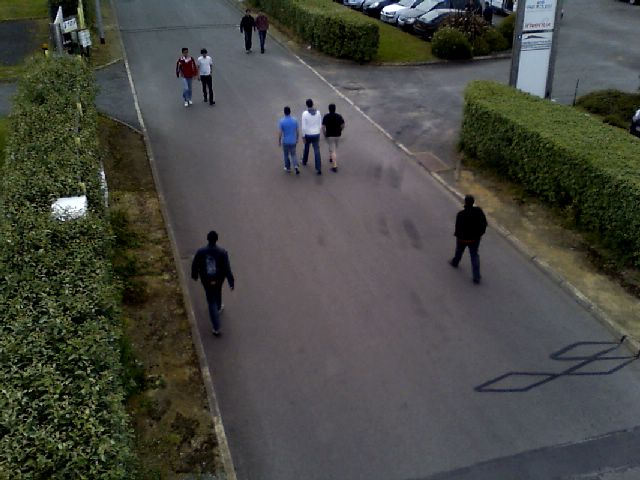
\includegraphics[scale=0.3]{Img/detection_0156}
		\end{center}
		\caption{Données d'entrée}
	\end{figure}
	
	Prenons une approche naïve. Le fond de l'image est fixe, les piétons sont les seuls objets en mouvement (en éliminant les mouvements parasites des feuilles et le bruit d'acquisition) : peut-on faire l'association objet en mouvement~$\Leftrightarrow $~piéton ? La partie \ref{sec:morpho} traite de cette approche.
	\\
	
	Mais les diverses études sur le sujet \ref{sec:bib} montrent que recourir au couple descripteur/classifieur augmente fortement la précision de l'algorithme. Nous avons donc également implémenté (voir partie \ref{sec:desc}) cette approche pour évaluer sa pertinence dans notre cas.

\section{APPROCHE MORPHOLOGIQUE}
\label{sec:morpho}

	A travers différentes opérations de filtrages non-linéaires par des éléments structurants, l'approche morphologique permet d'effectuer des traitements rudimentaires sur l'image. L'objectif est d'extraire des régions dans l'image (\emph{"blobs"} dans la documentation anglophone) en les séparant sur une image binaire.
	
	\subsection{Implémentation}
	Pour se détacher du fond il faut commencer par extraire le mouvement. Cela peut se faire par moyennage sur une plage d'images consécutives, par seuillage de la différence entre 2 images, par représentation probabiliste de chaque pixel, par création d'une image temporelle le long d'une ligne...
	
	Nous avons choisi d'implémenter l'approche morphologique avec cette dernière méthode. On définit donc une ligne de détection sur l'image, sur laquelle on élimine les pixels correspondant au fond par moyennage glissant sur 100 images. 
	On passe en image binaire par seuillage RGB réglable, afin de pouvoir appliquer les opérations morphologiques, qui se déroulent dans cet ordre :
	\begin{itemize}
	\item multiples itérations de l'opération $X_k = (X_{k-1} \oplus B) \cap A^c$ ("remplissage") jusqu'à ce que $X_k = X_{k-1}$. Cette opération sert à combler les trous.
	\item ouverture $X = (X \ominus B) \oplus B$. Cette opération supprime les éléments qui "dépassent".
	\end{itemize}
	
	\subsection{Identification}
	L'identification des régions se fait par analyse de connectivité sur l'image binaire obtenue : un filtre parcourt l'image pour associer un label à chaque groupe de pixels, puis un rapide traitement regroupe les labels coïncidents en blobs.
	
	
\section{APPROCHE DESCRIPTIVE}
\label{sec:desc}

	Le descripteur qui semble s'être imposé dans le domaine de la reconnaissance humaine de par sa relative simplicité (sans être le plus performant) est l'histogramme des gradients orientés (\emph{HOG}).
	
	Introduit et plébiscité par Dalal \& Triggs \cite{HOG} en 2005, l'HOG parcourt des cellules de petite taille, calcule le gradient (orientation + intensité) en chaque pixel, et crée un histogramme des orientations des gradients sur la cellule, pondérées par les intensités.
	
	\begin{figure}[hh]
		\begin{center}			
			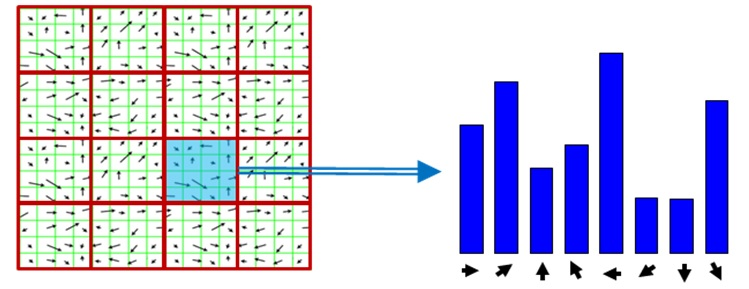
\includegraphics[scale=0.3]{Img/HOGtheory}
		\end{center}
		\caption{Principe de l'HOG}
	\end{figure}

	L'HOG donne de cette manière une bonne idée de la forme générale sur la cellule, et surtout quantifie cette information sur un nombre de directions et une précision en intensité réglables.
	
	\subsection{Implémentation}
	Pour appliquer ce descripteur, on parcourt l'image avec une fenêtre de taille fixe, décalée à chaque itération d'un certain pas, qui a son importance pour éviter les détections redondantes tout en maintenant une bonne précision. Pour gagner en temps de calcul, et simplifier la gestion de l'échelle variable entre arrière-plan et avant-plan, nous faisons parcourir cette fenêtre sur une zone prédéfinie (milieu de l'image) où l'échelle peut être considérée comme constante (on peut facilement s'affranchir de cette hypothèse en utilisant une fenêtre à taille variable).
	
	
	Le calcul de l'histogramme se fait sur des cellules, qui sont regroupées en blocs glissants sur lesquels on effectue une normalisation en norme 2 pour limiter les effets des changements de luminosité et de contraste sur l'image.
	L'histogramme calculé sur N valeurs de directions, donne donc un vecteur de taille M, avec 
	$$ M = NbBlocsParFenetre * TailleBloc * N $$
 	
	\subsection{Classification}

	Pour associer à chaque vecteur de taille M un label binaire d'appartenance à la classe "piétons", nous avons choisi d'utiliser une classification via SVM. A partir d'un set de données d'apprentissage (vecteurs de taille M) associées à un vecteur de classe binaire, la SVM (linéaire dans notre cas) détermine le meilleur hyperplan pour séparer ces deux classes dans l'espace de dimension M correspondant.
	
	L'apprentissage se fait avec des imagettes associées à des piétons et des imagettes associées au fond. Il est crucial d'être exhaustif dans cette phase d'apprentissage pour permettre à la SVM de gagner en sélectivité et donc en précision. Il a également été montré \cite{HOG} que les imagettes fournies à la SVM dans le cas de la détection de piétons doivent fournir une information de contexte, il faut donc laisser de la marge autour des piétons.
	
	\begin{figure}[h]
		\begin{center}			
			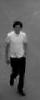
\includegraphics[scale=1]{Img/pieton_03}
		\end{center}
		\caption{Imagette d'apprentissage - piéton}
	\end{figure}
	
	
	\begin{figure}[h]
		\begin{center}			
			
\includegraphics[scale=1]{Img/fond_01}
		\end{center}
		\caption{Imagette d'apprentissage - fond}
	\end{figure}

\section{\'{E}valuation quantitative}
\label{sec:evalquant}

	\subsection{Méthodologie}
	Pour évaluer, opimiser et comparer les performances des algorithmes étudiés nous utiliserons l'outil classique de la matrice de confusion. Nous mesurons également le temps de calcul pour estimer la compatibilité avec une exécution temps réel (\emph{cf} partie \ref{sec:contexte}).
	
	\subsection{Résultats}
	
	\subsubsection{Comparaison des  descripteurs}	
	\label{sec:desccomp}
	Commençons par une comparaison via les matrice de confusion des descripteurs appliqués à une série de 200 imagettes correspondant soit à un piéton soit à du fond. La SVM est entraînée avec 20 imagettes.
	
	\begin{figure}[h]
		\centering
		\subfloat[HOG + SVM]{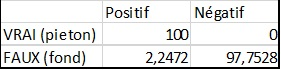
\includegraphics[scale=0.5]{Img/MATCONFHOGtest1}\label{fig:f1}}
		\hfill
		\subfloat[Morhpologie]{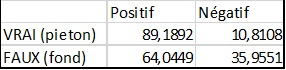
\includegraphics[scale=0.5]{Img/MATCONFMORPHOtest1}\label{fig:f2}}
		\caption{Matrices de confusion des descripteurs}
	\end{figure}
	
	L'histogramme des gradients est manifestement plus performant ici.
	
	\subsubsection{Influence du fond}
	Pour juger de l'influence du fond, nous répétons le test sur les mêmes imagettes mais avec un fond fixe (rue, pas de végétation).
	
	\begin{figure}[h]
		\centering
		\subfloat[HOG + SVM]{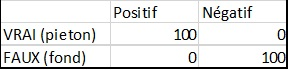
\includegraphics[scale=0.5]{Img/MATCONFHOGtest3}\label{fig:f1}}
		\hfill
		\subfloat[Morhpologie]{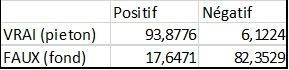
\includegraphics[scale=0.5]{Img/MATCONFMORPHOtest3}\label{fig:f2}}
		\caption{Influence du fond}
	\end{figure}

	On constate une nette amélioration de l'approche morphologique qui n'est plus perturbée par les pixels variables de la végétation, néanmoins les performances restent inférieures à celles du couple HOG+SVM.
	
	\subsubsection{Influence de l'apprentissage}
	Comme pressenti l'entraînement de la SVM influence les résultats, ci-dessous les résultats obtenus dans les mêmes conditions qu'au paragraphe \ref{sec:desccomp} mais avec un set d'apprentissage de 50 imagettes.
	
	\begin{figure}[h]
		\begin{center}			
			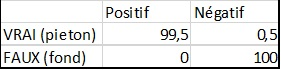
\includegraphics[scale=0.5]{Img/MATCONFHOGtest2}
		\end{center}
		\caption{Influence de l'apprentissage}
	\end{figure}
	Il y a effectivement une amélioration avec un plus grand set d'apprentissage, mais notons l'augmentation des faux négatifs dûs à une plus grande sélectivité, qui peut amener à rejeter des piétons.
	
		\begin{shaded}
			\textbf{Malgré de meilleures performances} sur le papier, le couple HOG+SVM s'est révélé trop conséquent en temps de caclul (de l'ordre de 1 IPS) dans l'implémentation sur Matlab pour le prototypage. Nous avons donc continué notre étude sur l'approche morphologique, en essayant d'optimiser les paramètres pour obtenir des performances satisfaisantes.
		\end{shaded}

	\subsubsection{Optimisation de la morphologie}
	Principalement 2 paramètres influent sur les performances de l'analyse morphologique :
	\begin{itemize}
		\item Le seuil d'intensité pour la conversion binaire de l'image RGB. Ce seuil peut être différent pour chaque couleur si le fond présente des propriétés particulières en couleur mais dans notre cas un seuil de gris est suffisant.
		\item Le type de l'élément structurant pour les opérations morphologiques
		\item La taille de l'élément structurant pour les opérations morphologiques
	\end{itemize}

	Ci-dessous les résultats obtenus sur une batterie de tests pour des images issues des données d'entrées, segmentées pour isoler la zone de passage des piétons (route), avec l'algorithme complet proposant un comptage de piétons :
	
	\begin{figure}[h]
		\centering
		\subfloat[\'{E}lément structurant discoïde]{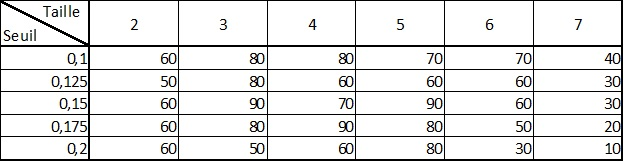
\includegraphics[scale=0.5]{Img/TRDISK}\label{fig:f1}}
		\hfill
		\subfloat[\'{E}lément structurant carré]{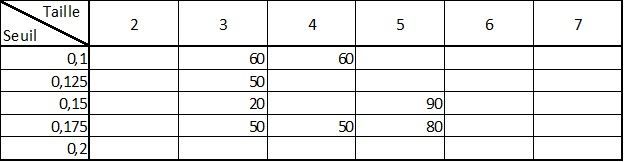
\includegraphics[scale=0.5]{Img/TRSQUARE}\label{fig:f2}}
		\caption{Tests d'optimisation}
	\end{figure}
	
	On obtient donc à priori des résultats optimaux pour un seuil de 0.175 et un masque discoïde de diamètre 3, de l'ordre de 90\% de précision.
	
	\subsubsection{Temps de calcul}
	Malgré quelques variations le temps de calcul reste relativement stable et donc indépendant des variations des paramètres. Ci-dessous des relevés pour différentes valeur de paramètres et un élément structurant en disque.
	
	\begin{figure}[h]
		\begin{center}			
			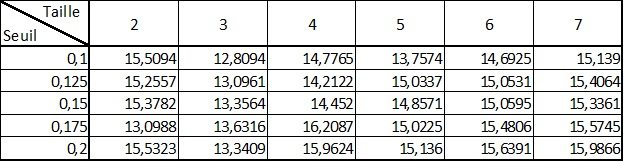
\includegraphics[scale=0.5]{Img/TPSDISK}
		\end{center}
		\caption{Temps de calcul (images par seconde)}
	\end{figure}
	On obtient un temps satisfaisant, qui répond correctement au cahier des charges (contrainte temps réel).
	
	
\section{Conclusion}
	
	Les résultats satisfaisants avec l'approche morphologique montrent que cette méthode peut se révéler pertinente dans notre cas. En effet, malgré une forte sensibilité aux situations complexes (végétation mouvante, groupe de piétons), il est possible d'optimiser le jeu de paramètres de manière à obtenir des résultats corrects. Le cas présent étant relativement simple dans son contexte, nous sommes convaincus que l'approche morphologique est la plus rentable en terme de temps de conception, de temps de calcul, de complexité, et de résultats, et mérite d'être considérée dans des cas similaires.
	\begin{figure}[hh]
		\begin{center}			
			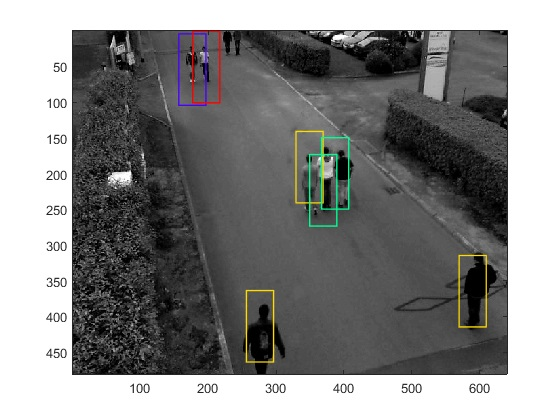
\includegraphics[scale=0.4]{Img/Identfications_Redondants}
		\end{center}
		\caption{Algorithme final de comptage}
	\end{figure}

	Cependant nous confirmons l'excellente performance du couple HOG + SVM qui se révèle très robuste, et peut s'adapter à toutes les situations avec un bon apprentissage. La difficulté est de trouver une manière efficace d'optimiser les calculs pour limiter le coût algorithmique, qui peut être conséquent si il faut parcourir toute l'image avec une fenêtre rectangulaire d'échelle variable. Cette méthode nécessite beaucoup d'étapes de traitements, toutes réglables avec un jeu de paramètres. Nous n'avons pas de doute sur la faisabilité de cette méthode dans notre cas, mais il faut alors utiliser un langage plus bas niveau et considérer un plus long temps d'étude pour parvenir à une solution répondant au cahier des charges.

\bibliographystyle{IEEEbib}
\bibliography{refs}

\end{document}
